\subsection{Market Risk}

\subsubsection{Value at Risk}

\begin{definition} \hlt{Value at Risk (VaR)}\\
Minimum loss expected a certain percentage of time over a certain time period given assumed market conditions.\\
Has three components: loss size, probability of loss greater than or equal to specified loss size, and time frame.\\
To estimate VaR, specify the time period. Given size of loss, estimate probability of loss. Given probability of loss, estimate minimum size of loss. VaR expressed for $1\%, 5\%, 16\%$. Time frame may be day, week, month etc.
\end{definition}

\begin{figure}[H]
\centering
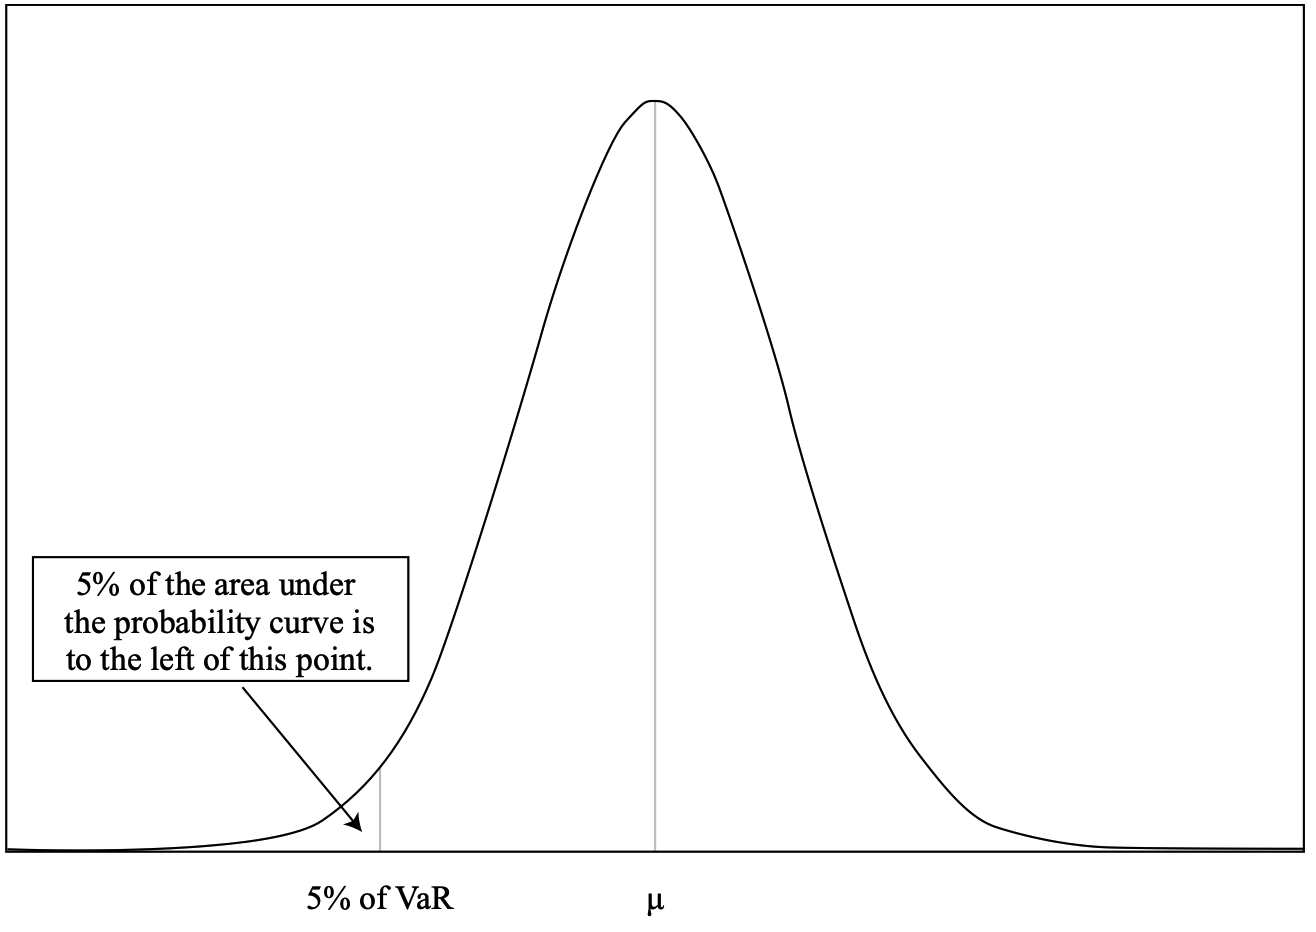
\includegraphics[scale=0.35]{/pm/fivepercvar}
\caption{$5\%$ VaR in context of probability distribution}
\end{figure}

\begin{method} \hlt{Steps of VaR Computation}
\begin{enumerate}[label=\roman*.]
\setlength{\itemsep}{0pt}
\item Use risk decomposition to identify factors, i.e., market risk, interest rate risk, currency risk, etc.
\item Gather data history for each of risk factors in VaR model (parametric, Monte Carlo, historical simulation)
\item Run the VaR models
\end{enumerate}
\end{method}

\begin{method} \hlt{Parametric Method}\\
Also known as analytical method or variance-covariance method.\\
Normal distribution is typically used, as only two parameters are required: expected value and standard deviation. Non-normality assumption would increase complexity of analysis due to more parameters required.\\
Expected return and volatility for a two asset ($A, B$) portfolio is then
\begin{align}
E(r_{\text{Portfolio}}) &= w_A E(r_A) + w_B E(r_B) \nonumber \\
\sigma_{\text{Portfolio}} &= \sqrt{w_A^2 \sigma_A^2 + w_B^2 \sigma_B^2 + 2 w_A w_B \rho_{A,B} \sigma_A \sigma_B} = \sqrt{w_A^2 \sigma_A^2 + w_B^2 \sigma_B^2 + 2 w_A w_B \text{Cov}(A,B)} \nonumber
\end{align}
where $w_A, w_B$ are weights; $E(r_A), E(r_B)$ are expected return; $\sigma_A, \sigma_B$ are volatility; $\rho_{A,B}$ is correlation.
Depending on time frame, $E(r_{\text{Portfolio}, 1 \text{ Day}}) = \frac{E(r_{\text{Portfolio}, n \text{ Days}}}{n}$, and $\sigma_{\text{Portfolio}, 1 \text{ Day}} = \frac{\sigma_{\text{Portfolio}, n \text{ Days}}}{\sqrt{n}}$.\\
Note that daily VaR cannot be annualised to annual VaR, as daily distribution of returns cannot be extrapolated to annual distribution; but we can annualise the data and estimate an annual VaR.\\
With portfolio standard deviation and standard normal statistics $z_{\alpha}$ for $\alpha \% $ VaR, portfolio VaR is then
\begin{align}
\text{VaR } \% &= \abs{E(r_{\text{Portfolio}}) = (\sigma_{\text{Portfolio}} \times z_{\alpha})} \nonumber \\
\text{VaR Value} &= \text{VaR } \% \times \text{Portfolio Value} \nonumber
\end{align}
\end{method}

\begin{remark} \hlt{Limitations of Parametric Method}\\
Although parametric method is simple to apply under assumption of normally distributed returns, estimates will only be as good as estimates of future mean returns and standard deviations.\\
Calculated VaR is very sensitive to covariance estimate. Length of lookback period will affect parameter estimates, and care must be taken to adjust estimates based on recent results, as future distributions may shift.\\
If normality cannot be assumed, i.e., portfolio contains options, parametric method is limited in usefulness.
\end{remark}

\begin{method} \hlt{Historical Simulation Method}\\
Based on actual periodic changes in risk factors over lookback period.\\
Changes in portfolio value are ordered, then largest $\alpha \%$ of losses are taken.\\
The smallest of these losses is the estimate of $\alpha \%$ VaR for the current portfolio.\\
No adjustments are made for difference between results for lookback period and that over a longer prior period.
\end{method}

\begin{remark} \hlt{Limitations of Historical Simulation Method}\\
No assumption of distribution is required to estimate VaR.\\
Method can be used to estimate VaR for portfolios with options.\\
VaR estimates depend on lookback period, and vary with characteristics of sample data used.\\
VaR based on high (low) volatility lookback period will yield overestimates (underestimates) of VaR.
\end{remark}

\begin{method} \hlt{Monte Carlo Simulation Method}\\
Simulation based on assumed probability distribution for each risk factor.\\
Assumption must be made about correlations between risk factors. Random values are generated for each risk factor, then pricing models used to calculate change in portfolio value for that set of risk factor changes.\\
Procedure is repeated thousands of times, outcomes ordered, then the $\alpha \%$ values are identified to estimate VaR.
\end{method}

\begin{remark} \hlt{Limitations of Monte Carlo Simulation}\\
Data used and assumptions about distributions of risk factors will have significant effects on estimated VaR.\\
Assuming large sample size, Monte Carlo method will produce identical results as the parametric method if distribution and parameters specified are the same.\\
Monte Carlo can accommodate virtually any distribution.
\end{remark}

\begin{remark} \hlt{Advantages of VaR}
\begin{enumerate}[label=\roman*.]
\setlength{\itemsep}{0pt}
\item Although methodology is technical, concept is simple and easy to explain
\item Allows comparison of risk of different portfolios, asset classes, or trading operations for relative riskiness
\item Used for performance evaluation through ratio of trading income to VaR
\item Used to allocate capital to various trading units by looking at allocation of VaR and optimising allocation of capital given maximum VaR that organisation should be exposed to (risk budgeting). Risk-adjusted performance of trading units or profits per dollar of VaR may be estimated.
\item Global banking regulators accept VaR as measure of financial risk, although there is no prescribed estimation methods or imposed maximum VaR
\item Reliability of VaR as measure of risk may be verified with backtesting
\end{enumerate}
\end{remark}

\begin{remark} \hlt{Limitations of VaR}
\begin{enumerate}[label=\roman*.]
\setlength{\itemsep}{0pt}
\item VaR estimations require many choices (loss percentage, lookback period, distribution assumptions, parameter estimates), and can vary significantly based on these choices.
\item Assumption of normality underestimates the tail risk as actual return distributions have fatter tails than normal distribution. Hence probability of extreme outcomes is underestimated.
\item Liquidity falls significantly when asset prices fall, which will understate actual losses incurred when liquidating positions under extreme price pressure.
\item Correlations increase or spike in times of financial stress. Increasing correlations meant VaR measures based on normal levels of correlation will overestimate diversification benefits and underestimate magnitude of potential losses.
\item Users of VaR must understand limitations of VaR as measure of risk to use it appropriately.
\item VaR focuses on downside risk and extreme negative outcomes only. Including right-hand tail values will hive better understanding of risk-return trade-off.
\end{enumerate}
\end{remark}

\begin{definition} \hlt{Conditional VaR (CVaR)}\\
Also known as expected tail loss or expected shortfall.\\
Expected loss, given that the loss is equal or greater than VaR.\\
In historical simulation method or Monte Carlo Method, this is average of all losses greater than VaR loss.\\
For parametric method, it is unknown for magnitude of losses greater than VaR, hence computing the expected loss in the left-hand tail is mathematically complex.
\end{definition}

\begin{definition} \hlt{Incremental VaR (IVaR)}\\
Change in VaR from a change in portfolio allocation to a security.\\
For example, assuming a $w \%$ increase in weight of security $A$, the VaR increased from $\$x$ to $\$y$, then the IVAR for $w \%$ increase in portfolio weight of security is $\$ (y - x)$.
\end{definition}

\begin{definition} \hlt{Marginal VaR (MVaR)}\\
Estimated as slope of curve that plots VaR as function of security's weight in portfolio.\\
Interpreted as change in VaR for a $1\%$ increase in security's weight.
\end{definition}

\begin{definition} \hlt{Ex Ante Tracking Error/Relative VaR}\\
Measure VaR of difference between return on portfolio and return on benchmark portfolio.\\
Computed as VaR of combination of long subject portfolio, short benchmark portfolio.\\
Interpreted as $\alpha \%$ of the time, portfolio underperformance will be at least $x \%$. 
\end{definition}

\subsubsection{Sensitivity Risk and Scenario Risk}

\begin{remark} \hlt{Sensitivity Analysis}\\
Focuses on effect on portfolio value given small change in one risk factor.\\
Complements VaR in understanding portfolio risk, but does not involve an prediction or probability of losses.
\end{remark}

\begin{remark} \hlt{Sensitivity Risk Measures}\\
Analysis portfolio exposure to various risk factors to facilitate risk management.\\
Factor sensitivities may be used to estimate effects of small changes in risk factors on securities.
\end{remark}

\begin{remark} \hlt{Scenario Analysis}\\
Estimates effect on portfolio value of a set of changes of significant magnitude in multiple risk factors.\\
Changes in risk factors are a set of changes that are expected to result in significant changes in portfolio value.
\begin{enumerate}[label=\roman*.]
\setlength{\itemsep}{0pt}
\item Historical Scenario: uses set of changes in risk factors that have occured in the past.
\item Hypothetical Scenario: uses set of changes in risk factors that may be more extreme than those that have occured in the past, but have some non-zero probability of occurring in the future.
\end{enumerate}
Usually final step in risk assessment and management process after sensitivity analysis.\\
For a firm that has limited its risk through maximum VaR, limits on position sizes, risk exposures etc, scenario analysis can provide additional information on portfolio vulnerability to a set of events or changes in correlations that would significantly reduce the value of the portfolio.
\end{remark}

\begin{remark} \hlt{Scenario Risk Measure}\\
Estimates portfolio return from a hypothetical market event or recurrence of a historical event.\\
Scenario analysis often performed as if scenario changes were instantaneous.\\
Scenario changes may be modelled as incremental changes, which includes portfolio manager actions in response to each change. This allow for reduction or closing of some positions or adjusting hedges appropriately. 
\end{remark}

\begin{remark} \hlt{Stress Test}\\
Examine effect on value or solvency of scenario of extreme risk-factor changes.\\
Firms that use leverage use stress tests involving a single risk factor to determine the size of change in factor that could result in losses such that the firm's sustainability is compromised.
\end{remark}

\begin{remark} \hlt{Reverse Stress Testing}\\
First step is to identify portfolio's largest risk exposures.\\
Next, an unacceptable outcomes is determined (usually scenario that threaten survival of an organisation), and scenarios of changes in risk factors that would result in such an outcome are identified.
\end{remark}

\begin{remark} \hlt{Sensitivity Risk Measure: Equity}\\
Primary equity exposure measure is beta, as measured by CAPM, extended by multi-factor models.
\begin{equation}
E[r_i] = r_f + \beta[E(r_m) - r_f] \nonumber
\end{equation}
\end{remark}

\begin{remark} \hlt{Sensitivity Risk Measure: Fixed Income}\\
Duration provides estimate of how market values are affected by changes in interest rates (YTM).\\
Convexity improves estimates of sensitivity of the values.
\begin{align}
\Delta B \approx -D \Delta y + \frac{1}{2} C (\Delta y)^2 \nonumber
\end{align}
where $\Delta B$ is change in bond price, $D$ is duration, $C$ is convexity, $\Delta y$ is change in YTM.\\
If duration used is Macaulay duration (instead of modified duration), then use $\frac{\Delta y}{1+y}$ in place of $\Delta y$.
\end{remark}

\begin{remark} \hlt{Sensitivity Risk Measure: Options}\\
Delta $\bm{\Delta}$ measures ratio of change in option value to change in price of underlying.\\
Gamma $\Gamma$ improves estimate of impact of change in price of underlying on option.\\
Vega $\mathcal{V}$ measures sensitivity of option values to changes in expected volatility of price of underlying.
\begin{equation}
\Delta P \approx \bm{\Delta} \Delta S + \frac{1}{2} \Gamma (\Delta S)^2 + \mathcal{V} \Delta V \nonumber
\end{equation}
where $\Delta P$ is change in price of option, $\Delta S$ is change in price of underlying, $\Delta V$ is change in future volatility.
\end{remark}

\begin{remark} \hlt{Advantages and Disadvantages of Risk Measures}\\
VaR, sensitivity analysis, scenario analysis complements each other, risk manager should not rely on only one.\\
VaR provides probability of loss. Sensitivity analysis provides estimates of relative exposures to different risk factors, but no estimate of probability of any specific changes in risk factors. Scenario analysis provide information to simultaneous changes in several risk factors or changes in risk correlations, but no probability associated with specific scenario other than empirical probability of historical scenario over look-back period.\\
In sensitivity analysis, even for two bond portfolios with same duration, yield volatility differs by portfolio and asset categories. Similarly, volatility of prices of underlying maybe different for different options.
\end{remark}

\subsubsection{Applications of Risk Measures}

\begin{remark} \hlt{Factors Influencing Type of Risk Measure Used}
\begin{enumerate}[label=\roman*.]
\setlength{\itemsep}{0pt}
\item Degree to which the market participant is leveraged, and need to assess minimum capitalisation and maximum leverage ratios
\item Mix of factors to which business is exposed (i.e., degree of equity or fixed income concentration in portfolios)
\item Accounting or regulatory requirements that govern reporting.
\end{enumerate}
\end{remark}

\begin{remark} \hlt{Use of Constraints to Limit Risk}\\
If constraints imposed are too restrictive, may impair profitability. If constraints are not restrictive enough, may lead to financial stress, corporate reorganisation, or bankruptcy.\\
Business-unit level restrictions may be too restrictive to the extent diversification benefits or offsetting positions across business units are not taken into account.
\end{remark}

\begin{remark} \hlt{Risk Limits: Risk Budgeting}\\
Risk management process that first determines acceptable total risk for an organisation, then allocates risk to different risk types (market, credit, operational) and different business units, geographies, and activities.
\end{remark}

\begin{remark} \hlt{Risk Limits: Position Limits}\\
Limits on market value of any instrument, or notional principal amount for a derivatives contract.\\
May also be limited on fronts such as: limits per issuer, per currency or country, on categories expected to be minimised in a given strategy, on gross size of long-short positions of derivatives activity, and on asset ownership that corresponds to market liquidity measures.\\
Do not take into account duration, volatility, correlation; controls for over-concentration.
\end{remark}

\begin{remark} \hlt{Risk Limits: Scenario Limits}\\
Limit on estimated loss for given portfolio, which if exceeded, would require corrective action on portfolio.
\end{remark}

\begin{remark} \hlt{Stop-Loss Limits}\\
Requires reduction in size of portfolio, or complete liquidation, when loss of particular size occurs in a specified period. Alternative is to impose requirement to undertake hedging activity, which include purchase of protective options, and increasing magnitude of hedge if losses increase.
\end{remark}

\begin{remark} \hlt{Capital Allocation Decisions}\\
Practice of placing limits on each of company's activities to ensure that areas in which it expects the greatest reward and has the greatest expertise are given the resources needed to accomplish their goals.\\
Optimal capital allocation, ignoring risk, the allocation that maximises expected return on invested capital. Risk management requires risk exposure for each use of firm capital to be considered.\\
To introduce risk exposures into decision making process, limit the overall risk of all activities. By calculating VaR for each activity or business unit, maximum acceptable VaR may be allocated accordingly.
\end{remark}

\begin{remark} \hlt{Risk Measures Used by Banks}\\
Banks may treat measures differently depending on accounting treatment.\\
Common to compute risk measures in distinct business units and geographies and then aggregate these measures to the parent company entity.
\begin{enumerate}[label=\roman*.]
\setlength{\itemsep}{0pt}
\item Liquidity Gap: extent of any liquidity and asset/liability mismatch. Ability to raise sufficient cash for foreseeable payment needs; view of liquidity of assets, expected repayment date of debt.
\item VaR: for held-for-sale or trading (fair value) portion of the balance sheet.
\item Leverage: computed, sometimes according to regulatory requirement or internally determined measure. Leverage ratios will weight risk assets using variety of methods and rules and divide this weighted asset figure by equity. Riskier assets will be assigned a greater weighting and less risky assets a lower weighting so that more equity is required to support riskier assets.
\item Sensitivities: for held-for-sale portion of balance sheet, uses duration, key rate duration or partial duration, and credit spread duration for interest rate risk positions. Also measure foreign exchange exposure and any equity or commodity exposures. All exposure measures will include delta sensitivities of options with any other exposures to same underlying, and will also monitor Gamma and Vega exposures of options. Gamma and Vega exposures can be broken out by term to identify how much of these risks come from long-dated versus short-dated options.
\item Economic Capital: measured by blending market, credit, and operational risk measures to estimate total loss the company could suffer at a very high level of confidence (e.g., $99\%$ to $99.99\%$), usually in one year’s time. Economic capital measures are applied to full balance sheet, including held-for-sale and held-for-investment portfolios, and include market, credit, and operational risk capital.
\item Scenario Analysis: stress tests applied to full balance sheet and augment economic capital and liquidity. Used to identify whether capital is sufficient for targeted, strong negative shocks. Outside of stress testing, significant scenario analysis takes places. Scenario analysis is used to examine how the full balance sheet might be affected by different interest rate, inflation, and credit environments, such as unemployment levels for credit card lenders, home price appreciation/depreciation for mortgage lenders, and business cycle stresses for corporate lenders.
\end{enumerate}
\end{remark}

\begin{remark} \hlt{Risk Measures Used by Asset Managers}\\
Focused primarily on volatility, probability of loss, or probability of underperforming a benchmark rather than insolvency. Each portfolio is measured with respect to its own constraints and limits. Exceptions:
\begin{enumerate}[label=\roman*.]
\setlength{\itemsep}{0pt}
\item Long-Only Asset Managers: if adviser has invested its own capital in any of the funds that it manages, these investments may need to be aggregated for the firm to assess its risk exposures across portfolios.
\item Hedge Funds: manager to aggregate adviser’s side-by-side investment in the various funds it advises.
\item Funds of Funds: risk measures for portfolios aggregate risks of underlying funds to master fund level.
\end{enumerate}
Manager may aggregate exposures across all funds and strategies to determine if there are unusual concentrations in individual securities or counterparties.
\end{remark}

\begin{remark} \hlt{Risk Measures Used by Long-Only Asset Managers}
\begin{enumerate}[label=\roman*.]
\setlength{\itemsep}{0pt}
\item Position Limits: include restrictions on country, currency, sector, and asset class; in absolute terms or relative to benchmark, as percentage of portfolio value.
\item Sensitivities: full range, including option-adjusted duration, key rate duration, and credit spread duration, and delta exposure of options in these measures. 
\item Beta Sensitivity: used for equity-only accounts
\item Liquidity: percentage of daily average trading volume the portfolio holds of each equity security and how many days it would take to liquidate a security 
\item Scenario Analysis: to verify that risks in the portfolio are as disclosed to investors and to identify any unusual behaviour that could arise in stressed markets.
\item Redemption risk: open-ended fund managers assess what percentage of the portfolio could be redeemed at peak times and track this behaviour across the funds and asset classes.
\item Ex Post versus Ex-ante Tracking Error: limits on ex ante tracking error are often used. Ex post tracking error to identify sources of performance and manager skill. Ex ante tracking error to identify if current positions could give rise to unexpected potential performance.\\
Active share to measure deviation from benchmark so as to monitor tracking error.
\item VaR: usually used by absolute-return managers.
\end{enumerate}
\end{remark}

\begin{remark} \hlt{Risk Measures Used by Hedge Fund Managers}
\begin{enumerate}[label=\roman*.]
\setlength{\itemsep}{0pt}
\item Sensitivities: full range of measures used
\item Gross Exposure: sum of the absolute value of long plus short positions. Long–short, market neutral, and arbitrage strategies measure long exposure, short exposure, and gross exposure separately.\\
Gross position risk measures correlation risk for the portfolio.
\item Leverage: to understand how the measure is treating derivatives, and components in numerator and denominator of the measure.
\item VaR: focus on high confidence intervals (more than $90\%$) and short holding periods
\item Scenarios: use scenario/stress tests that are well tuned to the specific risks of  strategy
\item Maximum Drawdown: worst-returning month or quarter for the portfolio or the worst peak-to-trough decline in a portfolio’s returns.
\end{enumerate}
\end{remark}

\begin{remark} \hlt{Risk Measures Used by Pension Funds}
\begin{enumerate}[label=\roman*.]
\setlength{\itemsep}{0pt}
\item Interest Rate and Curve Risk: expected future cash flows grouped by maturity, currency. Liability cash flows expressed as a short position at the relevant points on the curve.
\item Surplus at Risk: estimates how much the assets might underperform the liabilities. The more volatile the investments and the less well correlated these assets are with the liabilities, the higher the surplus at risk.
\item Liability Hedging Exposures versus Return Generating Exposures: precise instruments linked to the liability cannot always be directly invested in. A separate portion of the portfolio may be necessary and should perform the function of earning returns
\end{enumerate}
\end{remark}

\begin{remark} \hlt{Risk Measures Used by Property and Casualty Insurers}
\begin{enumerate}[label=\roman*.]
\setlength{\itemsep}{0pt}
\item Sensitivities and Exposures: insurers set asset allocation for these portfolios and monitor current exposures to remain within the target ranges set forth in the target asset allocation.
\item Economic Capital and VaR: risk modelling effort is to estimate what that catastrophic loss amount could be at a given level of probability. Assessment of the risk to economic capital will include the market risks in the portfolio as well as characteristics of the insurance exposures and reinsurance coverage.
\item Scenario Analysis: scenarios may stress the market risks and the insurance risks in the same scenario.
\end{enumerate}
\end{remark}

\begin{remark} \hlt{Risk Measures Used by Life Insurers}
\begin{enumerate}[label=\roman*.]
\setlength{\itemsep}{0pt}
\item Sensitivities: exposures of investment portfolio and annuity liability are measured and monitored.
\item Asset and Liability: investment portfolio is not designed to be a perfect match to the liabilities, but it is more closely matched to liabilities than in P\&C insurance.
\item Scenario Analysis: measures of potential stress losses based on the differences between the assets in which the insurance company has invested and the liabilities driven by the insurance contracts it has written to its customers. To stress both market and non-market sources of cash flow change.
\end{enumerate}
\end{remark}

\subsubsection{Backtesting and Simulations}

\begin{remark} \hlt{Backtesting}\\
Process of using historical data to emulate investment process and assess the risk and return.\\
Also helps investors to refine and improve investment process.\\
Relies on assumption that the future follows past trends to a degree.\\
Note, methodologies that perform well in backtest sometimes fail to deliver outperformance in actual use.
\end{remark}

\begin{remark} \hlt{Portfolio Construction Procedures}\\
Equity strategies typically use factor-based models, which represent unique sources of risk based on economic fundamentals. Goal of factor-based strategy is to identify signals to assemble portfolios that will outperform the overall market. To avoid data-mining trap, if a factor perform well in a backtest but doesn't have logical or economic reasoning backing it, the factor should be rejected. To formulate a theory and appropriate investing rules and procedures, then use historical data (training and sample) to measure performance.\\
It is more common to construct stock selection model that linearly combines several factors. Factor portfolios may be combined together with a benchmark portfolio (factors are weighted equally), or with risk parity portfolio (each factors contributes equally to risk).
\end{remark}

\begin{method} \hlt{Backtesting Process}
\begin{enumerate}[label=\roman*.]
\setlength{\itemsep}{0pt}
\item Strategy Design: identify investment goals and hypothesis.\\
For active strategy, goal is to achieve high risk-adjusted returns while managing downside risks.\\
Investment hypothesis is a method, which can be a trading rule, security selection criterion, portfolio etc.\\
Next, to transform hypothesis into rules and processes, specifying key parameters:
\begin{enumerate}[label=\arabic*.]
\setlength{\itemsep}{0pt}
\item Investment Universe: all assets which a position can be taken in while executing the strategy.
\item Definition of Return: either consolidated in local currency, or left as foreign currency. Choice of currency depends on whether the strategy requires hedging of currency exposures.\\
If goal is excess return, benchmark must be specified, which should relate to the investment universe.
\item Rebalancing Frequency and Transaction Cost: monthly rebalancing is typical, and higher frequencies are also common. Higher frequency rebalancing leads to higher transaction costs, and price data will be biased by bid-ask spreads, asynchronous trading across the world, missing days from holidays.\\
Consideration of transaction costs is crucial as market anomalies disappear when these are included.
\item Start and End Date: long data history is preferred to maximise confidence on the results.\\
Financial market data is non-stationary, hence likely to contain various distinct regimes. Hence, discrete time intervals should additionally be individually analysed.
\end{enumerate}
\item Historical Investment Simulation: portfolio is constructed and rebalanced according to predetermined frequency. Portfolio construction will be guided by investment strategy and constraints (geography, size, liquidity, limits on shorting).
\begin{enumerate}[label=\arabic*.]
\setlength{\itemsep}{0pt}
\item Rolling Window Backtesting: to evaluate viability of a factor, use a walk-forward (rolling window) system. Model parameters are fixed in advance to avoid overfitting. Strategy will be accepted if it performs well in out-of-test periods and makes logical sense.\\
Methodology implicitly assumes same pattern of past performance is expected to repeat over time. Results may not reflect dynamic nature of financial markets and possible extreme downside risk.
\item Backtesting Performance of Factor Allocation Strategies: to execute rolling window process twice. First, construct the factor portfolio using walk-forward approach, where each factor portfolios is long-short. Then use either benchmark or risk parity weighting to form a multi-factor portfolio. Then a second rolling window process is sued to determine covariances and create the risk parity portfolio. Both portfolios (which are long-only in terms of factor portfolios) are rebalanced monthly to maintain risk parity or equal weighting as appropriate. These portfolios are then analysed out-of-sample to determine returns on each portfolio.
\end{enumerate}
\item Analysis of Backtesting Output:
\begin{enumerate}[label=\arabic*.]
\setlength{\itemsep}{0pt}
\item Long-Short Hedged Portfolio Approach: from Fama French ($1993$). First, select a factor and rank investment universe by the factor in quantiles, and invest in each quantile based on a weighting scheme (equally or by market cap). Then long top quintile, short bottom quintile to form long-short hedged portfolio. Rolling window backtesting can then be applied, with portfolio rebalanced monthly. The series of out-of-sample performance data can then be analysed using metrics such as Value at Risk (VaR), Conditional Value at Risk (CVaR), Maximum Drawdown.
\item Comparing Results of Backtesting Methodologies: different backtesting methodologies may produce results that are different. There is no perfect methodology to use.\\
Ideally, multiple methods should suggest similar results
\end{enumerate}
\end{enumerate}
\end{method}

\begin{remark} \hlt{Issues in Strategy Backtesting}
\begin{enumerate}[label=\arabic*.]
\setlength{\itemsep}{0pt}
\item Survivorship Bias: driving conclusions from data that reflects only entities that have survived to date.\\
To use point-in-time data which is the most complete data for any given prior time period.\\
Entities may appear via IPOs, spin-offs, outperformance; entities may disappear due to privatisation, acquisition, prolonged under- or outperformance that changes market cap.
\item Look-Ahead Bias: from using data that was unknown or unavailable during historical periods over when the backtest was conducted. To use point-in-time data.\\
Reporting lag refers to situation where data describing a period is only available after the period ends.\\
Data revisions refers to situations where macro data are revised multiple times, companies restate financial statements. Databases only keep latest numbers.\\
Index addition is when data vendors add new companies to databases, and backtesting with current database will be using information on companies that were not in the database during backtesting period.
\item Data Snooping Bias: substituting sound portfolio construction by backtesting many strategies and choosing the best-performing strategy. Occurs when analysis is performed until a significant result is found.\\
Forms include performing interim analyses whether to continue collecting data, using many variables and deciding which to report later, dropping outliers only after performing analyses etc.\\
Mitigated by setting a much higher hurdle than typical critical $t$-statistics.\\
Alternatively, use cross-validation, such as rolling window backtesting.
\end{enumerate}
\end{remark}

\begin{remark} \hlt{Historical Scenario Analysis}\\
Backtesting of strategy on various regimes, taking into consideration the various structural breaks.\\
Typical types of regime change includes recession versus expansions, low versus high volatility periods, trade agreement and no-trade agreement environments.\\
Note risk and return of various strategies vary depending on the regime.\\
Probability density plot may reveal information on sensitivity of return distributions in different regimes.
\end{remark}

\begin{remark} \hlt{Historical Simulation}\\
Randomly draw past returns from long historical period, without order of occurrence. Similar to rolling-window backtesting, except the time sequence in which returns occured is not taken into account. Bootstrapping (random sampling with replacement) used if number of simulations required is larger than size of historical dataset.
\end{remark}

\begin{remark} \hlt{Monte Carlo Simulation}\\
Overcomes issue of only drawing from past data. Assigns statistical distribution from each variable, then draw random observations from this multivariate distribution, where parameters of the distribution are calibrated with past asset return data. Method is flexible, as it allows for a variety of distributions, catering for non-normality, tail dependence, fat tails etc. However, method is complex and requires significant computing power.\\
May be used to evaluate strategy's downside risk, and validate results of backtesting.
\end{remark}

\begin{method} \hlt{Steps of Simulation Analysis}
\begin{enumerate}[label=\arabic*.]
\setlength{\itemsep}{0pt}
\item Select target variable for analysis, typically return and its distribution
\item Specify key decisions variables, which are often returns of each underlying asset, weight.
\item Specify number of trials, typically between $1000$ and $10000$. The greater the number of trials, the more stable the predictions of performance and variance of performance.
\item Define distributional properties of each key variable, and also take tail dependence and correlations between variables into account.
\item Use random number generator to draw $N$ random numbers for each variable.
\item For each set of simulated key decision variables, compute the value.
\item Repeat steps $5$ to $6$ until completing desired number of trials ($N$).
\item Compute metrics of the $N$ simulated values of the target variable, such as mean, volatility, Sharpe ratio, various downside metrics (CVaR, maximum drawdown etc.)
\end{enumerate}
\end{method}

\begin{remark} \hlt{Sensitivity Analysis}\\
Enables understanding of how target variable varies due to changes in one of various input variables.\\
To quantify risk of misspecification, conduct sensitivity analysis by calibrating a different distribution to the factor return data, then running the process again.\\
Process is similar to that for Monte Carlo simulation, except data is fitted to multivariate $t$-distribution which allows for fat tails and skewness. After generating the samples, use risk measures such as Sharpe ratio or CVaR.
\end{remark}